%%%%%%%%%%%%%%%%%%%%%%%%%%%%%%%%%%%%%%%%%%%%%%%%%%%%%%%%%%%%%%%%%%%%%%%%%%%%%%%%%%%%%
%% Author: Sebastian Meyer <Sebastian.Meyer *a*t* ifspm *.* uzh *.* ch>
%%         based on the templates kindly provided by
%%         Daniel Sabanés Bové [daniel *.* sabanesbove *a*t* ifspm *.* uzh *.* ch]
%% Project: Journal Club Spring 2012
%%         
%% Time-stamp: <[talk.tex] by SM Fre 13/04/2012 12:50 (CEST)>
%%
%% Description:
%% Beamer template for the slidesf in the seminar.
%%
%% History:
%% 11/09/2009   file creation
%% 13/04/2012   adapted to the journal club
%%%%%%%%%%%%%%%%%%%%%%%%%%%%%%%%%%%%%%%%%%%%%%%%%%%%%%%%%%%%%%%%%%%%%%%%%%%%%%%%%%%%%

\documentclass[%
compress       % options for the beamer class
]{beamer}

% ----------------------------------------------------------------------
% choose language, coding and fonts
\usepackage[utf8]{inputenc}
\usepackage{textcomp}
\usepackage[english]{babel}
\usepackage[T1]{fontenc}
% ----------------------------------------------------------------------

% ----------------------------------------------------------------------
% other packages 
\usepackage{pgfpages}           % necessary for the handouts production
\usepackage{mathtools}           % for nice mathematics
\usepackage{bm}                 % bold math with \bm
\usepackage{booktabs}           % to make tables nicer
\usepackage{verbatim}           % for verbatim output
\usepackage{wasysym}            % symbols (smilies etc.)
\usepackage{natbib}    % for bibliography style and citations
\usepackage{transparent} %for writing transparent text
\usepackage{tikz} %for creating transparent rectangles etcs
\usepackage{multimedia}

% ----------------------------------------------------------------------
\usepackage{color}
\usepackage{amsmath, amssymb}
\usepackage{amsthm} %for proof env
\usepackage{multirow}
\usepackage{colortbl}
\usepackage{longtable}
\definecolor{grey}{rgb}{.95,.95,.95}
% ----------------------------------------------------------------------
% choose the beamer format: do not modify this
%%%%%%%%%%%%%%%%%%%%%%%%%%%%%%%%%%%%%%%%%%%%%%%%%%%%%%%%%%%%%%%%%%%%%%%%%%%%%%%%%%%%%
%% Author: Daniel Sabanés Bové [daniel *.* sabanesbove *a*t* ifspm *.* uzh *.* ch]
%% Project: Seminar Bayesian linear models
%%         
%% Time-stamp: <[format.tex] by DSB Mon 28/09/2009 16:06 (CEST)>
%%
%% Description:
%% Format for the beamer slides.
%%
%% History:
%% 11/09/2009   file creation: use slides layout by Andrea Riebler
%% 28/09/2009   add serif math font theme
%%%%%%%%%%%%%%%%%%%%%%%%%%%%%%%%%%%%%%%%%%%%%%%%%%%%%%%%%%%%%%%%%%%%%%%%%%%%%%%%%%%%%

% choose themes
\usetheme{Montpellier}
\usefonttheme[onlysmall]{structurebold}
\usefonttheme[onlymath]{serif}
\useoutertheme[subsection=false]{miniframes}

% modifications
\setbeamertemplate{bibliography item}[circle]
\setbeamertemplate{sections/subsections in toc}[sections numbered]
\setbeamertemplate{footline}{%
  \begin{beamercolorbox}[wd=\paperwidth,ht=0.25cm,center]{section in head/foot}
    \begin{beamercolorbox}[wd=0.38\paperwidth,ht=0.25cm,left]{section in head/foot}
      \raisebox{0.05cm}{\qquad \insertshortauthor}
    \end{beamercolorbox}
    \setbeamercolor{section in head/foot}{fg=white,bg=EPFL}
    \begin{beamercolorbox}[wd=0.53\paperwidth,ht=0.25cm, left]{section in head/foot}
      \raisebox{0.05cm}{\insertsubtitle}
    \end{beamercolorbox}
    \hskip-0.01\paperwidth
    \begin{beamercolorbox}[wd=0.04\paperwidth,ht=0.25cm,center]{section in head/foot}
      \raisebox{0.05cm}{\insertframenumber / \inserttotalframenumber}
    \end{beamercolorbox}
  \end{beamercolorbox}
} 

\beamertemplatenavigationsymbolsempty
\beamertemplateballitem

% colors
\definecolor{uzh}{RGB}{102,102,153}
\definecolor{EPFL}{RGB}{237,28,36}
\definecolor{biostat}{RGB}{46,191,199}
\definecolor{twitter}{RGB}{0,172,237}
\setbeamercolor{structure}{fg=twitter}
\setbeamercolor{palette quaternary}{bg=white,fg=twitter}
\setbeamercolor{section in head/foot}{bg=EPFL, fg=white}
\setbeamercolor{author in head/foot}{bg=white, fg=gray}
\setbeamercolor{titlelike}{parent=palette quaternary}
\setbeamercolor{item}{fg=twitter}
\setbeamercolor*{fine separation line}{fg=twitter}


%%% Local Variables: 
%%% mode: latex
%%% TeX-master: talk
%%% End: 

% ----------------------------------------------------------------------

% ----------------------------------------------------------------------
% FIXME: uncomment this to print the foils for handout:
% \pgfpagesuselayout{4 on 1}[a4paper,border shrink=5mm, landscape]
% ----------------------------------------------------------------------

%-----------------------------------------------------------------------
% specific options for tikz
%-----------------------------------------------------------------------

\usetikzlibrary{shapes,arrows,positioning}

\tikzset{decision/.style={diamond, draw, fill=black, text width=4.5em, text badly centered, inner sep=0pt}}
\tikzset{block/.style={rectangle, draw, fill=twitter, text width=5em, text centered, rounded corners,
 minimum width=3.5cm}}
\tikzset{sick/.style={rectangle, draw, fill=EPFL, text width=5em, text centered, rounded corners,
 minimum width=3.5cm}}
 \tikzset{healthy/.style={rectangle, draw, fill=green, text width=5em, text centered, rounded corners,
 minimum width=3.5cm}}
 \tikzset{decision2/.style={diamond, draw, fill=white, text width=4.5em, text badly centered, inner sep=0pt}}
\tikzset{basketball/.style={rectangle, draw, fill=white, text width=5em, text centered, rounded corners,
 minimum width=3.5cm}}
 \tikzset{flu/.style={rectangle, draw, fill=white, text width=5em, text centered, rounded corners,
 minimum width=3.5cm}}
\tikzset{line/.style={draw, -latex}}


% ----------------------------------------------------------------------
% FIXME: define the properties of the talk
\title{Does the Blue Bird get the Flu?}
\title{Weight of Statistical Evidence}
\subtitle{Detection and Correction of Publication Bias}
\author[Servan Grüninger]{Servan Grüninger\\
\bigskip
{\footnotesize Supervisor: Prof. Dr. Stephan Morgenthaler (EPFL)\\
External expert: Prof. Dr. Reinhard Furrer (University of Zurich)}}
\institute[shortinst]{Master's Programme in Computational Science and Engineering}
\vspace{0.5cm}
\date{Écublens, July 9th}
% ----------------------------------------------------------------------
% Set graphics path
% ----------------------------------------------------------------------
\graphicspath{{figures/}}

% ----------------------------------------------------------------------
% the document part:
% ----------------------------------------------------------------------
\usepackage{Sweave}
\begin{document}
\Sconcordance{concordance:EPFL_MasterThesis_Presentation.tex:EPFL_MasterThesis_Presentation.Rnw:%
1 100 1 1 0 5 1 1 7 2 1 1 5 375 1 1 27 16 1 1 7 5 0 1 7 1 2 500 1}

\setbeamertemplate{caption}{\raggedright\insertcaption\par}
\setbeamercovered{invisible}
\setkeys{Gin}{width=0.5\textwidth}





% title page
\frame[plain]{
\titlepage
\vspace{-1cm}
}

% outline page
\frame{
  \frametitle{Outline}
  \tableofcontents
}

% your contents: modify contents.tex
\section{Introduction and Goals}

\frame{
\frametitle{Publication Bias---The Bane of Scientific Publishing}
  \centering
  \begin{figure}[!htbp]
  \includegraphics[width= 0.7\textwidth]{PublicationBias.png}
  \caption{Many studies land in the file drawer (Image: \href{https://www.geckoboard.com/learn/data-literacy/statistical-fallacies/publication-bias/}{Geckoboard})}
  \end{figure}
}

\frame{
\frametitle{The Woozle Effect}
  \centering
  \begin{figure}[!htbp]
  \includegraphics[width= 0.5\textwidth]{WoozleEffect.png}
  \caption{\footnotesize{Pooh and Piglet tracking down the elusive Woozle (Image: Ernest H. Shepard)}}
  \end{figure}
}

\frame{
\frametitle{Influenza Surveillance in the USA}
\begin{itemize}
\item<1-> [] \textbf{Virology:} total \& influenza respiratory specimens per week
\item<2->  [] \textbf{ILI patients:} \% of total per week \& state
\item<3->  [] \textbf{Mortality:} influenza related deaths
\item<4->  [] \textbf{Hospitalisation:} influenza related hospitalisations
\item<5->  [] \textbf{Geographic spread of influenza:} within each state
\end{itemize}\bigskip
\raggedleft \tiny https://www.cdc.gov/flu/weekly/overview.htm
}

\frame{
\frametitle{Influenza Surveillance in the USA}
\textbf{Strengths:}
\begin{itemize}
\item reliable
\item comparably fast (ca. 1-2 weeks)
\item virological "ground truth"
\item severe cases covered
\end{itemize}\bigskip
\pause
\textbf{Weaknesses:}
\begin{itemize}
\item only tip of the iceberg
\item comparably slow (ca. 1-2 weeks)
\item weak cases are missed
\end{itemize}\bigskip
}

\frame{
\frametitle{Twitter as complementary information source}
\begin{itemize}
\item [] \transparent{0.5} \textbf{Virology:} total \& influenza respiratory specimens per week
\item [->] \transparent{1} \textbf{ILI patients:} \% of total per week \& state
\item [] \transparent{0.5} \textbf{Mortality:} influenza related deaths
\item [] \textbf{Hospitalisation:} influenza related hospitalisations
\item [->] \transparent{1} \textbf{Geographic spread of influenza:} within each state
\end{itemize}\bigskip
\raggedleft \tiny https://www.cdc.gov/flu/weekly/overview.htm
}

\frame{
\frametitle{Flu surveillance via twitter: two approaches}
\begin{columns}
  \column{0.5\textwidth}
  \centering
  correlate aggregated tweets with aggregated CDC data
  \begin{figure}[!htbp]
  \fbox{\includegraphics[width=0.9\textwidth]{figure/3_Bodnar2013.png}}
  \caption{\cite{bodnar_validating_2013}}
  \end{figure}
  % \raggedleft
  \pause
  \column{0.5\textwidth}
  \centering
  correlate individual tweets with disease state of individuals \textcolor{white}g
  \begin{figure}[!htbp]
  \fbox{\includegraphics[width=0.9\textwidth]{figure/4_ROC_classification_seed.png}}
  \caption{\cite{bodnar_ground_2014}}
  \end{figure}
\end{columns}
}

\frame{
\frametitle{Use aggregate data to detect the flu}
  \centering
  \begin{figure}[!htbp]
  \fbox{\includegraphics[width=0.9\textwidth]{figure/3_Bodnar2013.png}}
  \caption{\cite{bodnar_validating_2013}}
  \end{figure}
}

\frame{
\frametitle{Use aggregate data to detect the flu}
\textbf{Strengths:}
\begin{itemize}
\item "easy" with enough data
\end{itemize}\bigskip
\pause
\textbf{Weaknesses:}
\begin{itemize}
\item prone to overfitting
\item random data performed as good as tweets with flu related tweets
\item temporal \& spatial division of data influence model
\end{itemize}\bigskip
}

\frame{
\frametitle{The dangers of confounders}
\centering
\scalebox{1}{
      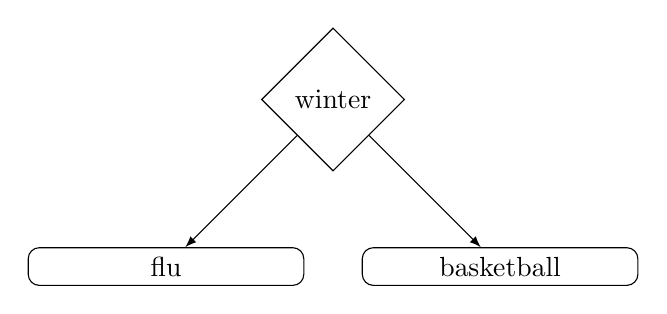
\begin{tikzpicture}[node distance=3cm]
        \node[decision2]   (nbrh){winter};
        \node[flu, below left of=nbrh](ovgt){flu};
        \node[basketball, below right of=nbrh]   (accp){basketball};

        \path[line] (nbrh) --          (ovgt);
        \path[line] (nbrh) --          (accp);
      \end{tikzpicture}%
}      
}


\frame{
\frametitle{The dangers of confounders}
\centering
\scalebox{1}{
      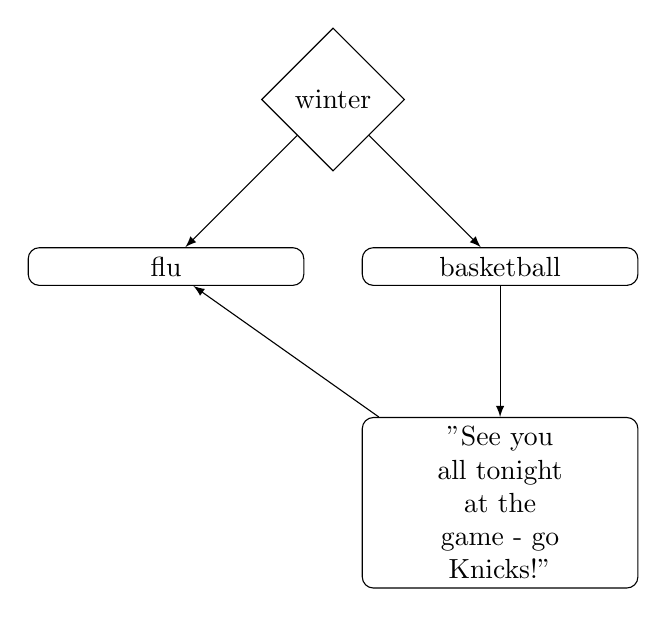
\begin{tikzpicture}[node distance=3cm]
        \node[decision2]   (nbrh){winter};
        \node[flu, below left of=nbrh](ovgt){flu};
        \node[basketball, below right of=nbrh]   (accp){basketball};
        \node[basketball, below of = accp] (bask){"See you all tonight at the game - go Knicks!"};        

        \path[line] (nbrh) --          (ovgt);
        \path[line] (nbrh) --          (accp);
        \path[line] (accp) --          (bask);
        \path[line] (bask) --      (ovgt);
      \end{tikzpicture}%
}      
}

\frame{
\frametitle{The cautionary tale of Google Flu Trends}
  \centering
  \begin{figure}[!htbp]
  \fbox{\includegraphics[width=0.9\textwidth]{figure/5_GFT.jpg}}
  \end{figure}
}

\frame{
\frametitle{Overfitting: The bane of machine learning}
  \centering
  \begin{figure}[!htbp]
  \fbox{\includegraphics[width=0.9\textwidth]{figure/3_Bodnar2013.png}}
  \caption{\cite{bodnar_validating_2013}}
  \end{figure}
}

\frame{
\frametitle{Flu surveillance via twitter: two approaches}
\begin{columns}
\column{0.5\textwidth}
  \centering
  \transparent{0.2} correlate aggregated tweets with aggregated CDC data
  \begin{figure}[!htbp]
  \fbox{\transparent{0.2}\includegraphics[width=0.9\textwidth]{figure/3_Bodnar2013.png}}
  \caption{\transparent{0.2}\cite{bodnar_validating_2013}}
  \end{figure}
  % \raggedleft
 \column{0.5\textwidth}
  \centering
  correlate individual tweets with disease state of individuals
  \begin{figure}[!htbp]
  \fbox{\includegraphics[width=0.9\textwidth]{figure/4_ROC_classification_seed.png}}
  \caption{\cite{bodnar_ground_2014}}
  \end{figure}
\end{columns}
}


\frame{
\frametitle{Use individual-level data to detect the flu}
\centering
\scalebox{1}{
      
\begin{tikzpicture}[node distance=3cm]
        \node[decision2] (init){Larry};

      \end{tikzpicture}%
}      
}

\frame{
\frametitle{Use individual-level data to detect the flu}
\centering
\scalebox{1}{
      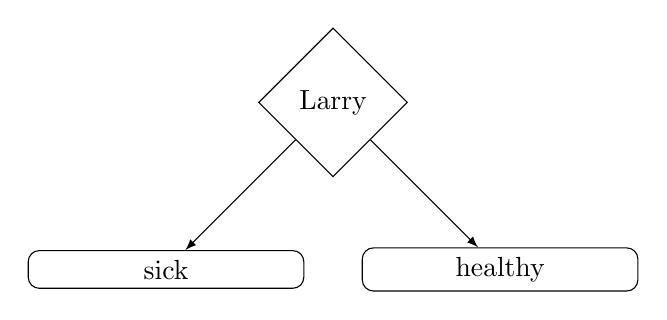
\begin{tikzpicture}[node distance=3cm]
        \node[decision2]   (nbrh){Larry};
        \node[basketball, below left of=nbrh](ovgt){sick};
        \node[basketball, below right of=nbrh]   (accp){healthy};

        \path[line] (nbrh) --          (ovgt);
        \path[line] (nbrh) --          (accp);
      \end{tikzpicture}%
}      
}

\frame{
\frametitle{Use individual-level data to detect the flu}
\centering
\scalebox{1}{
      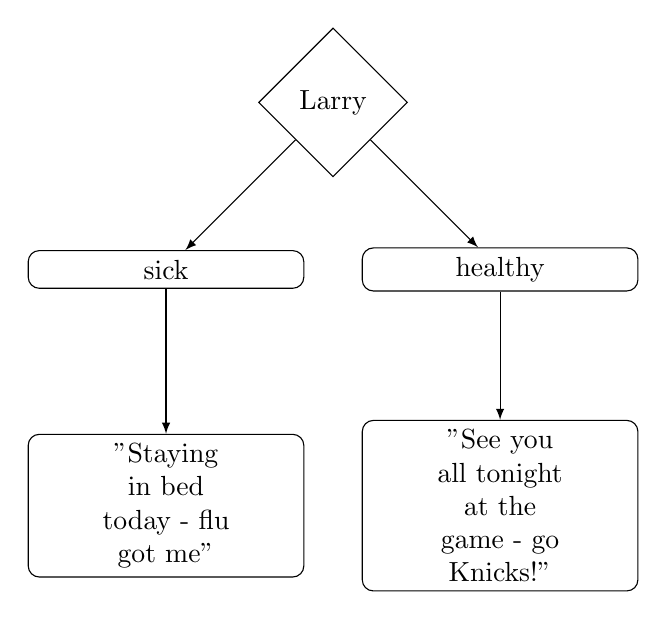
\begin{tikzpicture}[node distance=3cm]
        \node[decision2]   (nbrh){Larry};
        \node[basketball, below left of=nbrh](ovgt){sick};
        \node[basketball, below right of=nbrh]   (accp){healthy};
        \node[basketball, below of = accp] (bask){"See you all tonight at the game - go Knicks!"};
        \node[basketball, below of = ovgt] (flu){"Staying in bed today - flu got me"};

        \path[line] (nbrh) --          (ovgt);
        \path[line] (nbrh) --          (accp);
       \path[line] (accp) --          (bask);
        \path[line] (ovgt) --          (flu);

     \end{tikzpicture}%
}      
}


\frame{
\frametitle{On the ground validation of online diagnosis with Twitter and medical records \citep{bodnar_ground_2014}}
\begin{itemize}
\item 37'599 tweets from 104 accounts
\pause
\item 1609 tweets from 35 users w/ medically diagnosed flu in 2011/2012 season
\pause
\item ranked list of 12'393 most common keywords
\pause
\item rank established by different machine learning methods
\end{itemize}\bigskip
}

\frame{
  \begin{figure}[!htbp]
  \fbox{\includegraphics[width=0.9\textwidth]{figure/4_ROC_classification_seed.png}}
  \caption{\cite{bodnar_ground_2014}}
  \end{figure}
}

\frame{
\frametitle{The classifier model}
\begin{itemize}
\item naive Bayes classifier: $p(C_k \mid \mathbf{x}) = \frac{p(C_k) \ p(\mathbf{x} \mid C_k)}{p(\mathbf{x})}$
\item 100 most predictive keywords
\item accuracy: 89.72\%, AUC: 0.8544
\end{itemize}\bigskip
}

\frame{
\frametitle{Tweet classification: workflow}
\centering
\scalebox{1}{
      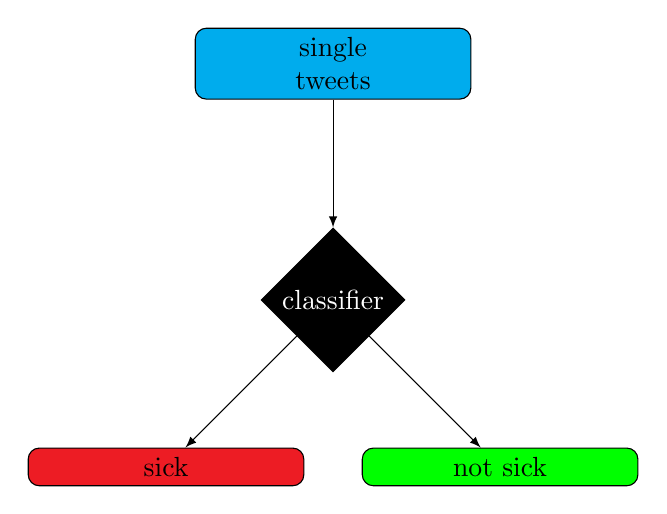
\begin{tikzpicture}[node distance=3cm]
        \node[block]                  (init){single tweets};
        \node[decision, below of=init]   (nbrh){\textcolor{white}{classifier}};
        \node[sick, below left of=nbrh](ovgt){sick};
        \node[healthy, below right of=nbrh]   (accp){not sick};

        \path[line] (init) --          (nbrh);
        \path[line] (nbrh) --          (ovgt);
        \path[line] (nbrh) --          (accp);
       
      \end{tikzpicture}%
}      
}

\frame{
\frametitle{Strengths and weaknesses of the Twitter classifier}
\textbf{Strengths:}
\begin{itemize}
\item "ground truth" available
\item high internal validity
\end{itemize}\bigskip
\pause
\textbf{Weaknesses:}
\begin{itemize}
\item small data set (-> low external validity?) 
  \begin{itemize}
  \item 104 individuals w/ influenza, 122 individuals w/o influenza 
  \item only 1609 tweets from 35 users in "sick" category
  \end{itemize}
\item low temporal resolution (one month time window)
\item ethical concerns (anonymity might be compromised)
\end{itemize}\bigskip
}

\frame{
\frametitle{Use individual data to detect the flu}
\transparent{0.2}\textbf{Strengths:}
\begin{itemize}
\item "ground truth" available
\item high internal validity
\end{itemize}\bigskip
\transparent{1}\textbf{Weaknesses:}
\begin{itemize}
\item small data set (-> low external validity?) 
  \begin{itemize}
  \transparent{0.2}\item 104 individuals w/ influenza, 122 individuals w/o influenza 
  \item only 1609 tweets from 35 users in “sick” category
  \end{itemize}
\transparent{1}\item low temporal resolution (one month time window)
\transparent{0.2}\item ethical concerns (anonymity might be compromised)
\end{itemize}\bigskip
}

\frame{
\frametitle{A first proof of principle}
  \begin{figure}[!htbp]
  \fbox{\includegraphics[width=0.8\textwidth]{figure/6_cdc_fit_bodnar_thesis.png}}
  \caption{\cite{bodnar_data_2015}}
  \end{figure}
}

\frame{
\frametitle{An adventure in reproducibility}
  \centering
  \begin{figure}[!htbp]
  \includegraphics[width= 0.7\textwidth]{figure/1_Reproducibility.jpg}
  \end{figure}
  http://blog.revolutionanalytics.com/2014/10/introducing-rrt.html
}

\frame{
\frametitle{To replicate or to reproduce?}
Reproducibility according to \cite{goodman_what_2016}:
\begin{itemize}
\item methods reproducibility
\item results reproducibility (replicability)
\item inferential reproducibility
\end{itemize}
}

\frame{
\frametitle{The three main goals:}
\begin{itemize}
\item Assess the validity of the Twitter classifier for large data sets (results and inferential reproducibility)
\bigskip
\item Reproduce key findings from \cite{bodnar_data_2015} (methods reproducibility)
\bigskip
\item Ensure the methods reproducibility of this thesis
\end{itemize}
}

\section{The Twitter Data Set}

\frame{

\centering
\bigskip
\huge \textbf{The Twitter Data Set}

}


\frame{
\frametitle{The nature of the data beast}
\begin{itemize}
  \item \texttt{all\_tweets}: the whole set of rated tweets (2'847'039'672~tweets)
  \item \texttt{one\_hundred}: the rated tweets of those users who sent at least 100 tweets (42'611'004~tweets)
  \item \texttt{sick\_users}: the rated tweets of all those users who sent at least one sick tweet (4'131'650~tweets)
\end{itemize}
}

\frame{
\frametitle{The nature of the data beast}
  \begin{figure}[!htbp]
  \includegraphics[width=0.8\textwidth]{figure/7_dataset.png}
  \end{figure}
}

\begin{Schunk}
\begin{Soutput}
         used (Mb) gc trigger  (Mb) max used  (Mb)
Ncells 409223 21.9     847687  45.3   641597  34.3
Vcells 828218  6.4   23885155 182.3 23324386 178.0
\end{Soutput}
\end{Schunk}

\frame{
\frametitle{The \texttt{sick\_users} data set - full}
  \begin{figure}[!htbp]
  \includegraphics[width=1\textwidth]{figure/8_all_tot_continent.png}
  \caption{4'131'650~tweets from 222'446 users before pre-processing}
  \end{figure}
}

\frame{
\frametitle{\texttt{sick\_users}: pruned tweets}
  \begin{figure}[!htbp]
  \includegraphics[width=1\textwidth]{figure/9_canexico_removed.png}
  \caption{3'696'989 tweets from 213'426 users after pre-processing}
  \end{figure}
}

\frame{
\frametitle{\texttt{sick\_users}: only few sick people in the data set}
  \begin{figure}[!htbp]
  \includegraphics[width=1\textwidth]{figure/10_barplot_sick_raw_df.pdf}
  \end{figure}
}

\frame{
\frametitle{\texttt{sick\_users}: differences between sick and healthy}
\begin{figure}[H]
\centering
\includegraphics[width=1\linewidth]{figure/11_user_activity_both_sick_raw_df.pdf}\newline
\caption{Mean = 16.01 (solid line); median = 12 (dashed line)}
\end{figure}
}

\frame{
\frametitle{\texttt{sick\_users}: differences between sick and healthy}
\begin{figure}[H]
\centering
\includegraphics[width=1\linewidth]{figure/12_user_activity_only_healthy_sick_raw_df.pdf}
\caption{Mean = 17.53 (solid line); median = 15 (dashed line)}
\end{figure}
}

\frame{
\frametitle{The \texttt{all\_tweets} data set}
\centering
  \begin{figure}[!htbp]
  \includegraphics[width=1\textwidth]{figure/13_activity_total_date_Twitter_full_aggregated.pdf}
  \caption{2'847'039'672 tweets sent by 16'015'981 users before pruning; 2'764'210'962 tweets and 15'229'049 users after pruning}
  \end{figure}
}

\frame{
\frametitle{\texttt{all\_tweets}: sick tweets over time}
  \centering
  \begin{figure}[!htbp]
  \includegraphics[width=1\textwidth]{figure/14_activity_sick_date_Twitter_full_aggregatedoverlay.pdf}
  \caption{1'189'809 sick tweets from max. 27'052 users}
  \end{figure}
}

\frame{
\frametitle{\texttt{all\_tweets}: sick users over time}
  \centering
  \begin{figure}[!htbp]
  \includegraphics[width=1\textwidth]{figure/15_activity_sick_user_date_Twitter_full_aggregatedoverlay.pdf}
  \end{figure}
}

\frame{
\frametitle{\texttt{all\_tweets}: total users over space}
  \centering
  \begin{figure}[!htbp]
  \includegraphics[width=1\textwidth]{figure/16_activity_total_user_state_Twitter_full_aggregated.pdf}
  \end{figure}
}

\frame{
\frametitle{\texttt{all\_tweets}: total users over space}
  \centering
  \begin{figure}[!htbp]
  \includegraphics[width=0.7\textwidth]{figure/17_ScatterTweetPop_user_log.pdf}
  \end{figure}
}

\frame{
\frametitle{\texttt{all\_tweets}: sick users over space}
  \centering
  \begin{figure}[!htbp]
  \includegraphics[width=1\textwidth]{figure/18_activity_sick_user_statename_Twitter_full_aggregatedoverlay.pdf}
  \end{figure}
}

\section{Competing for Gold}

\frame{

\centering
\bigskip
\huge \textbf{Competing For Gold}

}

\frame{
\frametitle{CDC ILI rates: the gold standard}
Influenza-like illnesses are defined as:
\begin{itemize}
\item fever (body temperature of 37.8°C or greater) AND
\pause
\item cough and/or sore throat AND
\pause
\item no other known cause
\end{itemize}

ILI rates are defined as the percentage of patients who visit ILINet sentinal clinics and show ILI symptoms.
}

\frame{
\frametitle{CDC vs. Twitter: tweet-based}
  \centering
  \begin{figure}[!htbp]
  \includegraphics[width=1\textwidth]{figure/19_cdc_twitter_comp_nat_raw.pdf}
  \caption{CDC ILI rates compared with Twitter sick tweet rate}
  \end{figure}
}

\frame{
\frametitle{CDC vs. Twitter: user-based}
  \centering
  \begin{figure}[!htbp]
  \includegraphics[width=1\textwidth]{figure/20_cdc_twitter_comp_nat_raw_user.pdf}
  \caption{CDC ILI rates compared with Twitter sick user rates}
  \end{figure}
}


\frame{
\frametitle{CDC vs. Twitter: normalised and user-based}
  \centering
  \begin{figure}[!htbp]
  \includegraphics[width=1\textwidth]{figure/21_cdc_twitter_comp_nat_ma1_user.pdf}
  \end{figure}
}

\frame{
\frametitle{CDC vs. Twitter: normalised, user-based, and smoothed}
  \centering
  \begin{figure}[!htbp]
  \includegraphics[width=1\textwidth]{figure/22_cdc_twitter_comp_nat_ma4_user.pdf}
  \end{figure}
}

\frame{
\frametitle{CDC flu activity levels}
\begin{itemize}
\item [0] insufficient data
\item [1] below baseline
\item [2] less than 1 SD above baseline
\item [3] less than 2 SD above baseline
\item [...]
\item [9] less than 8 SD above baseline
\item [10] more than 8 SD above baseline
\end{itemize}
}

\frame{
\frametitle{CDC flu activity levels - Baseline Calculation}

CDC calculation
\begin{itemize}
\item [] baseline =  $\frac{1}{n}\sum_{i=1}^{n} x_i + 2s$ \bigskip
\item [] \scriptsize $x_i$ = percentage of ILI patients among in week $i$; 
\item [] \scriptsize $n$ = \# of non-influenza weeks in previous three season
\item [] \scriptsize $s$ = sample standard deviation
\end{itemize}
\bigskip

\pause
adopted for Twitter data set
\begin{itemize}
\item [] baseline =  $\frac{1}{n}\sum_{i=1}^{n} x_i + 2s$ \bigskip
\item [] \scriptsize $x_i$ = number of tweets labelled "sick" in week $i$; 
\item [] \scriptsize $n$ = \# of non-influenza weeks in previous summer (Jun, Jul, Aug \& Sep)
\item [] \scriptsize $s$ = sample standard deviation
\end{itemize}
}

\frame{
\frametitle{CDC vs. Twitter: based on activity levels}
  \centering
  \begin{figure}[!htbp]
  \includegraphics[width=1\textwidth]{figure/23_cdc_twitter_comp_nat_activity_sick_user.pdf}
  \end{figure}
}


\frame{
\frametitle{CDC ILI activity levels: spatiotemporal activity}
\centering
\movie[height=0.7\textwidth, width = 0.9\textwidth, poster]{}{figure/24_regional_twitter_flu_full_national_rel_sick_user.avi}

}

\frame{
\frametitle{Twitter flu activity levels: spatiotemporal activity}
\centering
\movie[height=0.7\textwidth, width = 0.9\textwidth, poster]{}{figure/25_regional_twitter_flu_full_rel_sick_user.avi}
}

\frame{
\frametitle{CDC vs. Twitter: spatiotemporal comparison}
\centering
\movie[height=0.7\textwidth, width = 0.9\textwidth, poster]{}{figure/26_regional_Twitter_cdc_diff_full_rel_sick_user.avi}
}

\section{Exercises in Reproducibility}

\frame{

\centering
\bigskip
\huge \textbf{Exercises in Reproducibility}

}

\frame{
\frametitle{Reproducing key figures from \cite{bodnar_data_2015}}
\begin{itemize}
\item SIR model parameters $\beta$ and $\gamma$
\pause
\item SIR model figure
\pause
\item full Twitter model figure
\end{itemize}
}

\frame{
\frametitle{SIR model in \cite{bodnar_data_2015}}
  \centering
  \begin{figure}[!htbp]
  \includegraphics[width=1\textwidth]{figure/26_todd_bodnar_SIR.png}
  \caption{SIR model based on yearly (solid) and combined (dashed) parameters}
  \end{figure}
}

\frame{
\frametitle{SIR model theory}
\begin{itemize}
\item $\frac{dS}{dt} = -SI\beta$\bigskip
\pause
\item $\frac{dI}{dt} = -SI\beta - I\gamma$\bigskip
\pause
\item $\frac{dR}{dt} = I\gamma$\bigskip
\end{itemize}
\pause

$\beta$ and $\gamma$ are estimated by minimising the residual sum of squares:
$$\text{RSS} = \sum_{t}(I_{\gamma, \beta}(t)-I_{\text{CDC}}(t))$$
}

\frame{
\frametitle{SIR model: data basis for calculation}

\begin{itemize}
  \item \texttt{cdcoffset}
 \item \texttt{full\_base}
  \item \texttt{full\_autocor}
  \item \texttt{full\_autocor2}
  \item \texttt{full\_both} 
  \item \texttt{full\_both2}
\end{itemize}

Optimisation done with a simple grid-search algorithm.
}

\frame{
\frametitle{National best-fit parameters from the CDC (white) and Twitter data (grey)}
\begin{table}[H]
\centering
\begin{tabular}{l l l l l}
 Year & \(\gamma\) & \(\beta\) & RSS\\ \hline
& 0.4 & 0.44  & 0.00041   \\ 
 {\multirow{-2}{*}{ 2011-2012 (Bod)}}  & \cellcolor{grey}0.37  & \cellcolor{grey}0.41 & \cellcolor{grey}0.00036  \\ \cline{2-4}
 \pause
    {\multirow{2}{*}{ 2011-2012 (Gru) }}& 0.17 & 0.17  & 0.00010   \\ 
   & \cellcolor{grey}0.12  & \cellcolor{grey}0.12  & \cellcolor{grey}0.00013  \\ \cline{2-4}
\end{tabular}
\end{table}
}

\frame{
\frametitle{SIR model in \cite{bodnar_data_2015}}
  \centering
  \begin{figure}[!htbp]
  \includegraphics[width=1\textwidth]{figure/26_todd_bodnar_SIR.png}
  \caption{SIR model based on yearly (solid) and combined (dashed) parameters}
  \end{figure}
}

\frame{
\frametitle{SIR model: based on \texttt{cdcoffset}}
  \centering
  \begin{figure}[!htbp]
  \includegraphics[width=1\textwidth]{figure/27_SIR_model_cdc_data_25.pdf}
  \caption{}
  \end{figure}
}

\frame{
\frametitle{SIR model: based on \texttt{full\_both2}}
  \centering
  \begin{figure}[!htbp]
  \includegraphics[width=1\textwidth]{figure/28_SIR_model_full_model_25.pdf}
  \caption{Full model consisting of AR(2) model based on CDC data and Twitter base model}
  \end{figure}
}

\frame{
\frametitle{Full Twitter model from \cite{bodnar_data_2015}}
  \begin{figure}[!htbp]
  \fbox{\includegraphics[width=0.8\textwidth]{figure/6_cdc_fit_bodnar_thesis.png}}
  \caption{\cite{bodnar_data_2015}}
  \end{figure}
}

\frame{
\frametitle{Full Twitter model from \cite{bodnar_data_2015}}

$$I_{\text{full}}(t + 1) = a \cdot I_{\text{CDC}}(t - 1) + b \cdot I_{\text{CDC}}(t) + c \cdot I_{\text{Twitter}}(t) + d.$$
}


\frame{
\frametitle{Full Twitter model from  \cite{bodnar_data_2015}}
  \centering
  \begin{figure}[!htbp]
  \includegraphics[width=1\textwidth]{figure/29_SIR_model_full_both_25_colorised.pdf}
  \caption{Full model consisting of AR(2) model based on CDC data and Twitter base model}
  \end{figure}
}

\frame{
\frametitle{CDC AR(2) model}
  \centering
  \begin{figure}[!htbp]
  \includegraphics[width=1\textwidth]{figure/30_SIR_model_full_AR2_100_colorised.pdf}
  \caption{Model consisting of AR(2) model based on CDC data }
  \end{figure}
}

\frame{
\frametitle{Twitter base model}
  \centering
  \begin{figure}[!htbp]
  \includegraphics[width=1\textwidth]{figure/31_SIR_model_full_base_model_100_colorised.pdf}
  \caption{}
  \end{figure}
}

\frame{
\frametitle{CDC vs. Twitter: user-based}
  \centering
  \begin{figure}[!htbp]
  \includegraphics[width=1\textwidth]{figure/20_cdc_twitter_comp_nat_raw_user.pdf}
  \caption{CDC ILI rates compared with Twitter sick user rates}
  \end{figure}
}

\section{Discussion}

\frame{

\centering
\bigskip
\huge \textbf{Discussion}

}

\frame{
\frametitle{Discrepancies between Grüninger [2017] and \cite{bodnar_data_2015}}
With regard to: \bigskip
\begin{itemize}
\item methods reproducibility: figures \& tables not reproducible
\pause
\item results reproducibility: Classifier results did not fit CDC rates
\pause
\item inferential reproducibility: Classifer detects flu peaks, but is only of complementary use
\end{itemize}\bigskip
\pause
Most likely explanation: Data set used by \cite{bodnar_data_2015} was pruned, filtered, or otherwise transformed.
}

\frame{
\frametitle{Support for "Transformation hypothesis"}
\begin{itemize}
\item stark discrepancies with regard to basic parameters of the two dat sets (e.g. mean tweets sent, total number of users, relative distribution of sick users )
\end{itemize}
}


\frame{
\frametitle{Differences in data sets}
\begin{table}[H]
\centering
\begin{tabular}{l l l l l}
  & Bodnar  & Grüninger & Note\\ \hline
\# users  & 15'560'328 & 15'229'049 & raw   \\ 
\pause
\# tweets  & 2'732'174'105 & 2'847'039'672 & raw   \\ 
\pause
\# sick users (2011-2015) & 182'801 & 27'052 & processed \\
\pause
mean tweet rate & 175.59 tw/pp & 31.42 tw/pp &  per week \\
\pause
median tweet rate & 10 tw/pp & 32.53 tw/pp &  per week \\
\pause
\# total users in 2011 & 45'086 & 175'382 & processed \\
\end{tabular}

\end{table}

}

\frame{
\frametitle{Support for "Transformation hypothesis"}
\begin{itemize}
\item stark discrepancies with regard to basic parameters of the two dat sets (e.g. mean tweets sent, total number of users, relative distribution of sick users )
\item sick rates in \cite{bodnar_data_2015} were 10-times larger than in my set
\item \texttt{sick\_user} subset
\end{itemize}
}

\frame{
\frametitle{Discrepancies between Grüninger [2017] and \cite{bodnar_data_2015}}
With regard to: \bigskip
\begin{itemize}
\item methods reproducibility: figures \& tables not reproducible
\item results reproducibility: Classifier results did not fit CDC rates
\item inferential reproducibility: Classifer detects flu peaks, but is only of complementary use
\end{itemize}\bigskip
Another explanation: Data set used by \cite{bodnar_data_2015} was the same, but there were crucial gaps and/or fundamental errors in reporting.
}

\frame{
\frametitle{Why not to trust Grüninger [2017]?}
\begin{itemize}
\item no possibility to re-run classifier
\pause
\item large, unwieldy data-set, analysed by novice data scientist
\pause
\item no access to complete code and processed data base used by \cite{bodnar_data_2015}
\end{itemize}
}

\frame{
\frametitle{Why to trust Grüninger [2017]?}
\begin{itemize}
\item analysed \& aggregated data in various ways (spatial, temporal) and with various methods
\pause
\item key statistics of aggregated data resemble real-world Twitter statistics more closely
\pause
\item Because the literature and \cite{bodnar_data_2015} say so
\end{itemize}
}

\frame{
\frametitle{Recommendations}
\begin{itemize}
\item Assessing validity of analysis of Grüninger [2017]
\pause
\item re-establishing functionality of Twitter classifier
\pause
\item testing classifier with representative subset of Twitter users
\end{itemize}
}

\frame{

\centering
\bigskip
\huge \textbf{Stop.}

}

% the bibliography
%\newcommand{\newblock}{}            % uncomment this line if there is an error complaining about an unknown command
\begin{frame}[allowframebreaks]
  \frametitle{References}
  \vspace{-0.5cm}
  \footnotesize
  \bibliographystyle{unsrtnat}
  \bibliography{Papers.bib}
\end{frame}

\end{document}
% ----------------------------------------------------------------------


% Local Variables:
% mode: latex
% coding: utf-8-unix
% End:
